%% Please fill in your name and collaboration statement here.
\newcommand{\studentName}{Kevin Zhang}
\newcommand{\collaborationStatement}{I collaborated with Tomoya Hasegawa, Annie Hwang and Jessica Zhu, got help from no one else, and referred to no other sources.}


%%%%%%%%%%%%%%%%%%%%%%%%%%%%%%%%%%%%%%%%%%%%%%%
\documentclass[solution, letterpaper]{cs121}
\usepackage{enumerate}
\usepackage{tikz}
\usepackage{pgf}
\usepackage{tikz}
\usetikzlibrary{arrows,automata}
\usepackage{hyperref}
\usetikzlibrary{automata,positioning}
\begin{document}
\header{4}{Due October 20, 2015 11:59pm}


%%%%%%%%%%%%%%%%%%%%%%%%%%%%%%%%%%%%%%%%%%%%%%%
\PART{Zhengyu and Sam}
%%%%%%%%%%%%%%%%%%%%%%%%%%%%%%%%%%%%%%%%%%%%%%%



\problem{3+3+3} {1/2 page}
For each of the following languages, state whether the language is context-free or not. If context-free, give a context-free grammar that generates the language (or construct a pushdown automaton that recognizes the language). If not context-free, write a short proof to justify.

\subproblem $\{a^{n} : n \text{ is a prime number}\}$. 
\subproblem $\{a^nb^m : n,m\in \mathbb{N},  n \neq m\; \textrm{and}\; n \neq 2m\}$.
\subproblem
$\{a^{n}b^{n}c^{n} : n\in\mathbb{N}\} \cup \{(ab)^n(ca)^n(cb)^n : n\in\mathbb{N}\}$. 

\begin{solution}
\subsolution The pumping lemma for CFL's states that if $L$ is a CFL, then it has a pumping length $p$ such that every string $s \in L, |s| \ge p$ can be written as $uvxyz$, where $|vy| > 0$ and $|vxy| \le p$ such that $uv^ixy^iz \in L$ for all $i \in \mathbb{N}$.  In this case, suppose the given language is a CFL.  Say we have a string $s$ in the given language with pumping length $p$.  The pumping lemma tells us that $s$ can be written in some satisfactory form $uvxyz$; suppose $n = |vy|$ and $m = |uxz|$.  Then pumping $s$ tells us that $m + ni$ must be a prime for all $i \in \mathbb{N}$.  But this is obviously not true; simply take the value $i = m$ to get the length $m + nm = m(n+1)$, which is not prime.  Hence, the given language cannot be a CFL, and we are done.
\subsolution This is a context free language.  To prove this, we construct three separate grammars for each of the cases $n < m$, $n \in (m, 2m)$, and $n > 2m$, then union them; since CFLs are closed under union, the result will be a CFL as well.  In the following cases, $V = \{S, A, B\}$, $E = \{a, b\}$, and $S = \{S\}$.  The three $R$'s are given as follows:
\begin{itemize}
	\item $n < m$.  Then $R$ is given by $\{S \mapsto Ab, A \mapsto Ab | B, B \mapsto aBb | \vareps\}$.  It is not hard to see that this guarantees that the number of $b$'s is always larger than the number of $a$'s here, as desired.
	\item $n \in (m, 2m)$.  Then $R$ is given by $\{S \mapsto aaaAbb, A \mapsto BaAb | \vareps, B \mapsto a | \vareps \}$.  Let's walk through this mathematically.  First, $m \ge 2$; if $m$ is any less, there are no valid strings.  Hence, we require that the string have at least $3$ $a$'s and $2$ $b$'s, as in the first rule (if $m \ge 2$, then $n > 2$).  Next, we allow the insertion of equal numbers of $B$'s, $a$'s, and $b$'s, as in the second rule.  This ensures that the number of $a$'s is still greater than the number of $b$'s; i.e. $n > m$.  Lastly, we replace every $B$ with either an $a$ or a $\vareps$.  Let us walk through the math here; suppose the second rule is invoked $k$ times.  Then the number of $b$'s as a result is exactly $k+2$, the number of $B$'s is exactly $k$, and the number of $a$'s is exactly $k + 3$.  The third rule allows us to replace all $B$'s with however many $a$'s we want; in simpler terms, we can take out all the $B$'s we have and replace them with at most as many $a$'s that we want.  But then this means that the final number of $a$'s is between $k+3$ and $2k+3$, or in the range $(k+2, 2(k+2)) = (m, 2m)$ as required.
	\item $n > 2m$.  Then $R$ is given by $\{S \mapsto aA, A \mapsto aA | B, B \mapsto aaBb | \vareps\}$.  It is not hard to see that this guarantees that $n > 2m$; the last rule guarantees $n \ge 2m$, and the first and second rule force insertion of at least 1 more $a$ at the beginning.
\end{itemize}

The above three sets of rules generate the desired languages; unioning them gives the desired result.

\subsolution Assume this language is a CFL, and let the pumping length be $p$.  Consider the string $a^pb^pc^p$.  Note that no matter what we pump, as long as we pump $v$ and $y$ at least once the resulting string will begin with at least two $a$'s; this means that it cannot be in the second half of the union that this language is defined by (namely, it is not any string in $(ab)^n(ca)^n(cb)^n$, which must either start with $ab$ or be the empty string).  But the canonical proof for showing that $a^nb^nc^n$ already showed that pumping this string always results in a string that is not of the form $a^nb^nc^n$; hence, pumping $a^pb^pc^p$ results in multiple strings that are not in either $a^nb^nc^n$ or $(ab)^n(ca)^n(cb)^n$, and we are done.
\end{solution}


\problem{6}{1/2 page}
Draw the state diagram of a PDA that recognizes the language $\{w :$ the number
of $a$'s in $w$ is greater than two times the number of $b$'s in $w\}$. Use
Sipser's notation to label the transitions. (That is, use labels in the form
$x,y\to z$ to mean that when you read an $x$ from your string and pop a $y$
from the stack, follow the transition and push a $z$ onto the stack.) Explain
in a few sentences why your construction is correct (no need to prove
formally).

\begin{solution}
\begin{center}
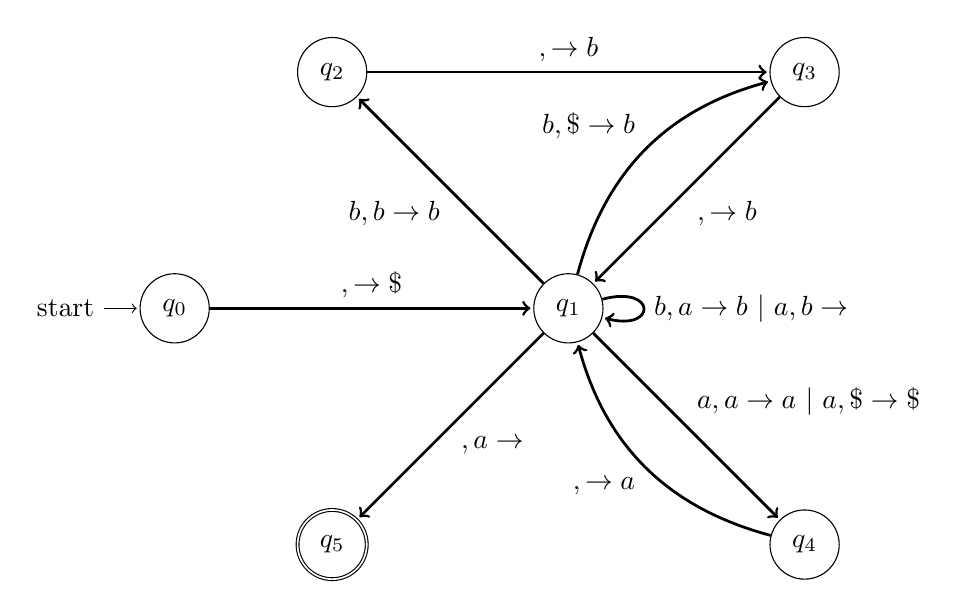
\begin{tikzpicture}[shorten >=1pt,node distance=3cm,on grid,auto] 
	\node[state, initial] 		(q_0) 						{$q_0$};
	\node[state] 			(q_1) [right=of q_0, xshift = 2cm] 				{$q_1$};
	\node[state]			(q_2) [above=of q_1, xshift = -3cm]	{$q_2$};
	\node[state]			(q_3) [above=of q_1, xshift = 3cm]	{$q_3$};
	\node[state]			(q_4) [below=of q_1, xshift = 3cm]	{$q_4$};
	\node[state, accepting]	(q_5) [below=of q_1, xshift = -3cm]	{$q_5$};  

\path[->, line width=1pt]
	(q_0) 	edge 			node {$\vareps, \vareps \rightarrow \$$}				(q_1)
	(q_1)		edge				node {$b, b \rightarrow b$}							(q_2)
			edge [bend left]		node {$b, \$ \rightarrow b$}							(q_3)
			edge				node {$a, a \rightarrow a$ $|$ $a, \$ \rightarrow \$$}		(q_4)
			edge [loop right]		node {$b, a \rightarrow b$ $|$ $a, b \rightarrow \vareps$}	()
			edge				node {$\vareps, a \rightarrow \vareps$}				(q_5)
	(q_2)		edge				node {$\vareps, \vareps \rightarrow b$}				(q_3)	
	(q_3)		edge				node {$\vareps, \vareps \rightarrow b$}				(q_1)
	(q_4)		edge	[bend left]		node {$\vareps, \vareps \rightarrow a$}				(q_1)
;

\end{tikzpicture}
\end{center}

This solution works by increasing a quantity $k$ by 2 whenever it reads a $b$ from the input tape and decreasing it by 1 whenever it reads an $a$; $k$ here represents the number of $a$'s minus twice the number of $b$'s.  At any point, we non-deterministically allow a transition from $q_1$ to an accept state by popping an $a$ off the stack; if any characters are left on the input tape, the PDA will fail because there are no transitions out of said accept state.  Thus, this transition can only occur if there is a $a$ on the stack at the very end; the logic transitioning out of $q_1$ ensures that this only occurs if $k > 0$.
\end{solution}


\problem{6}{1/2 page}
A pushdown automaton (PDA) is made by equipping an NFA with a stack. In this
problem, we consider an NFA equipped with a queue -- a Queue Automaton (QA).
The queue supports the following two operations:
\begin{enumerate}
  \item {\em Pop.} Read the leftmost symbol of the queue and remove it from
    the queue.
  \item {\em Push.} Write a symbol to the rightmost end of the queue.
\end{enumerate}

In a Queue Automaton, a transition $(q, \sigma, \gamma)\rightarrow (q',
\gamma')$ means ``if the machine is in state $q$, after reading $\sigma$ from
the input string and popping $\gamma$ from the queue, push
$\gamma'$ onto the queue and transition to state $q'$''. Note that
$\varepsilon$-transitions are still allowed. For example, $(q, \varepsilon,
\gamma)\rightarrow (q', \gamma')$ doesn't read anything from the input string.
You can also use an $\varepsilon$ for $\gamma$ to indicate that nothing should
be popped from the queue, and an $\varepsilon$ for $\gamma'$ to indicate that
nothing should be pushed onto the queue. Initially the queue is empty.

We saw in class that $L=\{a^{2^n} : n \in \Nat \}$ is not Context-Free, so
there isn't a PDA that recognizes it. Construct a Queue Automaton that {\em
does} recognize $L$ (give the 6-tuple for it) and provide a short explanation
for why it works.

\begin{solution}
We give the Queue Automaton as follows: $Q = \{S, q_1, q_2, F\}$, $\Sigma = \{a\}$, $\Gamma = \{A, a\}$, $q_0 = S$, $F = F$, and $\gamma$ as follows:
\begin{center}
\begin{table}[h!]
	\begin{center}
		\begin{tabular}{ c | c | c | c | c}
			$q$ & $\sigma$ & $\gamma$ & $q'$ & $\gamma'$\\
			\hline
			$S$ & $a$ & $\vareps$ & $q_1$ & $A$\\
			$q_1$ & $a$ & $A$ & $q_2$ & $A$\\
			$q_1$ & $a$ & $a$ & $q_2$ & $a$\\
			$q_1$ & $\vareps$ & $A$ & $F$ & $\vareps$\\
			$q_2$ & $\vareps$ & $\vareps$ & $q_1$ & $a$\\
		\end{tabular}
	\end{center}
\end{table}

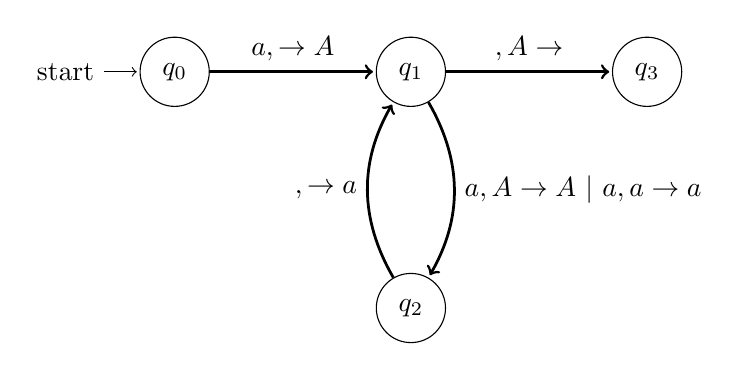
\begin{tikzpicture}[shorten >=1pt,node distance=3cm,on grid,auto] 
	\node[state, initial] 		(q_0) 						{$q_0$};
	\node[state] 			(q_1) [right=of q_0] 				{$q_1$};
	\node[state]			(q_2) [below=of q_1]				{$q_2$};
	\node[state]			(q_3) [right=of q_1]				{$q_3$};

\path[->, line width=1pt]
	(q_0) 	edge 			node {$a, \vareps \rightarrow A$}					(q_1)
	(q_1)		edge	[bend left]		node {$a, A \rightarrow A$ $|$ $a, a \rightarrow a$}	(q_2)
			edge				node {$\vareps, A \rightarrow \vareps$}			(q_3)
	(q_2)		edge	[bend left]		node {$\vareps, \vareps \rightarrow a$}			(q_1)	
;

\end{tikzpicture}
\end{center}

This works by keeping track of the number of $a$'s left until the next power of 2 by keeping that number of $a$'s at the top of the queue.  For example, the queue would consist of the values $\{A\}$, $\{A, a\}$, $\{a, A, a\}$, $\{A, a, a, a\}$, $\{a, a, a, A, a\}$, and so on, as $a$'s were read in consecutively.  At each step, the number of $a$'s preceding the $A$ (note there is only ever one $A$ in the queue) represents the number of $a$'s left until the next power of 2.
\end{solution}



%%%%%%%%%%%%%%%%%%%%%%%%%%%%%%%%%%%%%%%%%%%%%%%
\PART{Charles and Serena}
%%%%%%%%%%%%%%%%%%%%%%%%%%%%%%%%%%%%%%%%%%%%%%%


\problem{4+6+(2)}{1 page}
Recall that allowing nondeterminism did not add any power to finite 
automata---any language that could be accepted by an NFA could also be 
accepted by a DFA. In this problem, you will show that this is \emph{not 
the case} for PDAs by defining Deterministic PDAs (DPDAs). \\ 

DPDAs are similar to PDAs with a few subtle differences: 
\begin{itemize}
\item Most notably, they are deterministic in their transitions and
  stack operations.  Note that this means that they don't allow
  transitions on $\varepsilon$.  In one step, a DPDA reads exactly one
  input symbol, reads and pops exactly one symbol from the top of the
  stack, and pushes a {\em string} onto the stack.
\item Instead of starting with an empty stack, they start with a
  special symbol, $\$$, as the lone symbol on the stack. This way a
  DPDA can always know when it has reached the bottom of its
  stack. The $\$$ symbol can never be erased; that is, any transition
  reading $\$$ \emph{must} push it back on the stack.
\end{itemize}

\subproblem  Formalize the above by definining a DPDA as a 7-tuple $(Q,
\Sigma, \Gamma, \$, \delta, q_0, F)$, filling in the requirements of
each component.  You can refer to the definitions of a regular PDA for
the components that don't change.
\subproblem Now you will show that DPDAs are more powerful than finite automata. Consider the language $\textsc{Majority} =\{w: w \text{ contains more
$a$'s than  $b$'s}\}$. Construct a DPDA that recognizes $\textsc{Majority}$. Prove that no finite automata recognizes $\textsc{Majority}$.
\subproblem (CHALLENGE!!! Optional, worth 2 extra points.) Show that DPDAs are less powerful than PDAs.

\begin{solution}
\subsolution A DPDA consists of a PDA with an added component, the \$, and long with several requirements: 
\begin{itemize}
	\item $Q$ is the set of states,
	\item $\Sigma_\vareps$ is the input alphabet (which contains $\vareps$),
	\item $\Gamma_\vareps$ is the stack alphabet (which must always contain \$),
	\item \$ is the initial symbol on the stack,
	\item $\delta: Q \times \Sigma_\vareps \times \Gamma_\vareps \rightarrow (Q \times \Gamma^*) \cup \{\emptyset\}$ is the transition function ($\Gamma^*$ refers to any string constructed from the stack alphabet),
	\item $q_0 \in Q$ is the start state, and
	\item $F \subseteq Q$ is the set of accept states.
\end{itemize}

In addition, there are three restrictions on the transition function $\delta$: it can only take in $\vareps$ for either of its inputs for $\Sigma$ or $\Gamma$ if no subsequent transition could be combined with the $\vareps$ transition; if its input for $\Gamma$ is \$, the returned value for $\Gamma^*$ must contain \$ somewhere in the string, and the returned values are well defined for any triple $(q, \sigma, \gamma) \in Q \times \Sigma_\vareps \times \Gamma_\vareps$ (that is, there is only one possible output of $\delta$ for every input triple).

\subsolution The DPDA is given by this diagram:
\begin{center}
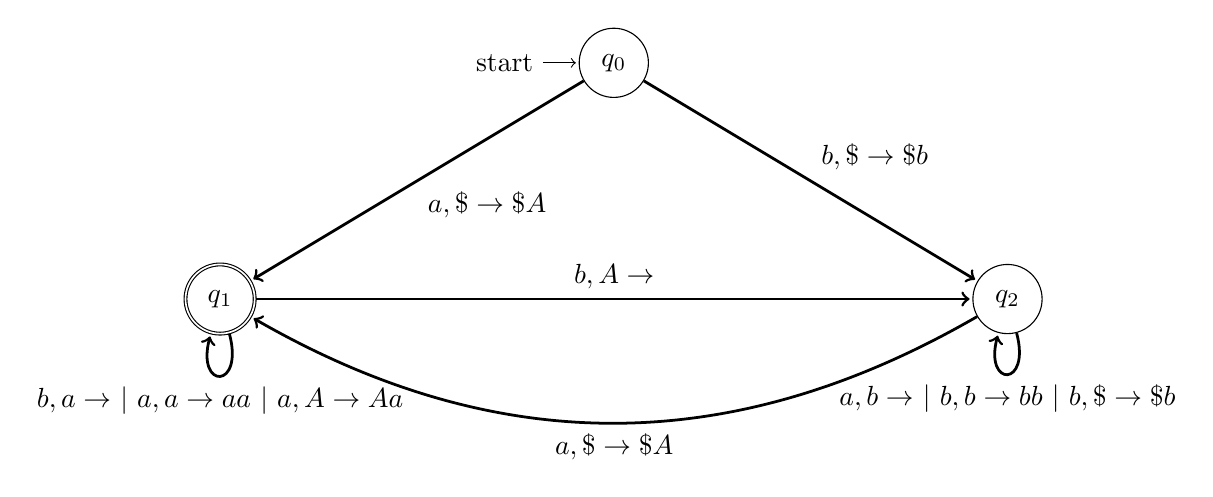
\begin{tikzpicture}[shorten >=1pt,node distance=3cm,on grid,auto] 
	\node[state, initial] 		(q_0) 						{$q_0$};
	\node[state, accepting] 	(q_1) [below=of q_0, xshift = -5cm] 	{$q_1$};
	\node[state]			(q_2) [below=of q_0, xshift = 5cm]	{$q_2$};

\path[->, line width=1pt]
	(q_0) 	edge 			node {$a, \$ \rightarrow \$A$}					(q_1)
			edge				node	{$b, \$ \rightarrow \$b$}					(q_2)
	(q_1)		edge				node {$b, A \rightarrow \vareps$}					(q_2)
			edge	[loop below]	node {$b, a \rightarrow \vareps$ $|$ $a, a \rightarrow aa$ $|$ $a, A \rightarrow Aa$}	()
	(q_2)		edge	[bend left]		node {$a, \$ \rightarrow \$A$}					(q_1)	
			edge [loop below] 	node {$a, b \rightarrow \vareps$ $|$ $b, b \rightarrow bb$ $|$ $b, \$ \rightarrow \$b$}	()
;
\end{tikzpicture}
\end{center}

where the stack alphabet is $\{\$, a, b, A\}$ and the input alphabet is $\{a, b\}$.  This works by keeping track of the difference in the number of $a$'s and $b$'s, and keeping track of the first $a$ that is pushed on the stack (this is required because of the deterministic construction).

Proving that no finite automata accepts this language is easy using the pumping lemma; suppose that this language is regular (i.e. a finite automata accepts it) and let its pumping length be $p$.  Consider $b^pa^{p+1}$.  Deconstructing this string into components $xyz$ that satisfy the pumping lemma, we see that since $|xy| \le p$, $xy$ must consist entirely of $b$'s.  But then since $|y| > 0$, $y$ must be at least one $b$; pumping $y$ results in strings that have at least as many $b$'s than $a$'s; i.e. it results in strings that aren't in this language.  Hence, this language cannot be regular, and it is not accepted by any finite automata.

\subsolution The intuitive approach, where we try to find a language which we can prove is in one set but not the other, is hard to do in this case.  How do we prove that a language requires nondeterminism?  Instead, we find a property of DPDAs that some PDAs do not have.

One special property of DFAs was that swapping all of the reject and accept states resulted in a DFA that accepted the exact complement of the language described by the initial DFA.  The same is true for DPDAs; any deterministic sequence of transitions that results in an accept state would now result in a rejection, and any sequence that results in a reject state would now result in an accept.  This is true because there is exactly one sequence of transitions for any well-defined DPDA.  For a NPDA, this is not true; a NPDA only requires that one of the possible sequences of transitions results in an accept state, so if one possible sequence for an input $s$ ends in an accept state and another possible sequence ends in a reject state, flipping the states results in a NPDA that still accepts $s$.  

This implies that every DCFL's (a language accepted by a DPDA) complement must also be a DCFL.  But then if we manage to find a CFL whose complement isn't a CFL, then it cannot be a DCFL (since DCFLs are all CFLs as well).  But we already know this is possible, since CFLs are not closed under complementation; hence, DCFLs are a strict subset of CFLs, and therefore DPDAs are weaker than PDAs in general.
\end{solution}

\problem{8}{3/4 page}
If $L$ is a language, then {\sc Permutation}$(L) = \{ x:
$ there exists a string $w \in L$ such that $|x|=|w|$ and the number
of occurrences of any letter in $w$ and $x$ are the same$\}$. Show
that if $L$ is regular, then {\sc Permutation}(L) is context free
when $\Sigma = \{a, b\}$. (Hint: Your proof must use the fact that there are only two symbols in the alphabet---the proof does not generalize to the case $\lvert \Sigma\rvert >2$.)

\begin{solution}
Since $L$ is regular, it must have a DFA that accepts it.  Let's call that DFA $D$.  We can construct a PDA that accepts $Permutation(L)$; let $V = \{\$, -, +\}$, $\Sigma = \{a,b\}$, $S = \$$, and define the transitions as follows:
\begin{itemize}
	\setlength\itemsep{0cm}
	\item Begin with a start state for the PDA, and draw a transition on $\vareps, \vareps \rightarrow \$$ to the start state of $D$.
	\item Draw a final state, and draw transitions from every final state of $D$ to this final state on $\vareps, \$ \rightarrow \vareps$.
	\item Replace every final state originally in $D$ with a non-final state.
	\item We need to fix the transitions in $D$; note that each transition acts on $a$ or $b$ in $D$.  We'll fix them as follows:
	\begin{itemize}
		\item Transitions on $a$.  Replace with the set of rules, $a, \vareps \rightarrow \vareps$ $|$ $b, \$ \rightarrow -$ $|$ $b, - \rightarrow --$ $|$ $b, + \rightarrow \vareps$.
		\item Transitions on $b$.  Replace with the set of rules $b, \vareps \rightarrow \vareps$ $|$ $a, \$ \rightarrow +$ $|$ $a, + \rightarrow ++$ $|$ $a, - \rightarrow \vareps$.
	\end{itemize}
\end{itemize}

The basic idea behind this PDA is to mirror a DFA that accepts $L$ and keep track of the error in the value defined by as the number of $a$'s minus the number of $b$'s read so far from the input string.  E.g., if we are at a state in the DFA where we have read the string $ab$, but the string $aa$ has been fed into the PDA, the error in $($\#$a) - ($\#$b)$ would be +1, since we have seen two $a$'s and zero $b$'s when instead we should have seen one of each.  We define two quantities: $X$, the number of $a$'s minus the number of $b$'s read so far at any state in the ORIGINAL DFA (i.e. the value of $($\#$a)-($\#$b)$ that we should have so far), and $Y$, the number of $a$'s minus the number of $b$'s so far in the PDA that we have defined above (i.e. the value of $($\#$a)-($\#$b)$ in the PDA so far).  We claim that $X - Y$ is exactly $0$ whenever we reach a final state of the DFA.

\indent To see this, consider the example string $aaababb$, and the test string $aabbbaa$.  Comparing these two strings one character at a time, we see that the pair of values $(X,Y)$ follows the sequence $(1, 1), (2, 2), (3, 1), (2, 0), (3, -1), (2, 0), (1, 1)$.  More accurately, the quantity $X - Y$ follows the sequence $0, 0, 2, 2, 4, 2, 0$.  Now consider the other string $aabbbab$; the quantity $X - Y$ follows the sequence $0, 0, 2, 2, 4, 2, 2$.  Now to prove this formally; first of all, note that strings must have the same length to be permutations of each other.  Next, note that if two strings of the same length have the same number of $a$'s, then they have the same number of $b$'s as well, and if they have the same number of $a$'s and $b$'s then they are permutations of one another.  To be more exact, if two strings have the same length and the values $($\#$a) - ($\#$b)$ is the same for both, then they are permutations of one another - but this is exactly the condition $X = Y$!  
\indent Now let's see how our stack models this.  First of all, our stack consists of three objects; $\$$, $+$, and $-$.  We'll use our stack to keep track of the quantity $X - Y$.  In our stack, if the top symbol is a $\$$ then $X - Y = 0$.  If the stack consists of a $\$$ and $k$ $+$'s, then $X - Y = -2k$ (that is, we have read $k$ more $a$'s instead of $b$'s than we were supposed to so far).  Similarly, if the stack consists of a $\$$ and $k$ $-$'s, then $X - Y = 2k$ (we have read $k$ more $b$'s instead of $a$'s than we were supposed to so far).  Using these definitions then, we take $X - Y = 0$ to mean that we have read exactly the correct number of $a$'s and $b$'s so far.

\indent The above construction is probably best demonstrated using a DFA and its constructed PDA.  Consider this DFA and PDA:
\begin{center}
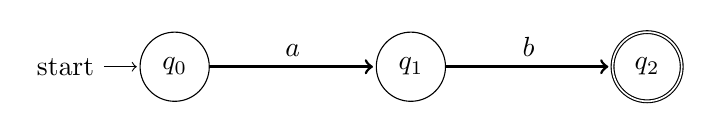
\begin{tikzpicture}[shorten >=1pt,node distance=3cm,on grid,auto] 
	\node[state, initial] 		(q_0) 				{$q_0$};
	\node[state] 			(q_1) [right=of q_0] 		{$q_1$};
	\node[state, accepting]	(q_2) [right=of q_1]		{$q_2$};

\path[->, line width=1pt]
	(q_0) 	edge 			node {$a$}					(q_1)
	(q_1)		edge				node {$b$}					(q_2)
;
\end{tikzpicture}

\vspace{0.5cm}

\begin{tikzpicture}[shorten >= 1pt,node distance=3cm, on grid, auto]
	\node[state, initial]		(q_0')				{$q_0'$};
	\node[state]			(q_0) [right=of q_0']		{$q_0$};
	\node[state]			(q_1) [below=of q_0]		{$q_1$};
	\node[state]			(q_2) [below=of q_1]		{$q_2$};
	\node[state, accepting]	(q_f) [left=of q_2]		{$q_f$};

\path[->, line width=1pt]
	(q_0')	edge				node {$\vareps, \vareps \rightarrow \$$}		(q_0)
	(q_0)		edge				node {$a, \vareps \rightarrow \vareps$ $|$ $b, \$ \rightarrow -$ $|$ $b, - \rightarrow --$ $|$ $b, + \rightarrow \vareps$}												(q_1)
	(q_1)		edge				node {$b, \vareps \rightarrow \vareps$ $|$ $a, \$ \rightarrow +$ $|$ $a, + \rightarrow ++$ $|$ $a, - \rightarrow \vareps$}												(q_2)
	(q_2)		edge				node {$\vareps, \$ \rightarrow \vareps$}		(q_f)
;
\end{tikzpicture}
\end{center}

The DFA accepts the language $\{ab\}$.  Let's walk through the PDA with $ba$ and with $aa$.  With $ba$, the only transitions we can make consist of $\vareps, \vareps \rightarrow \$$, then $b, \$ \rightarrow -$, then $a, - \rightarrow \vareps$, then $\vareps, \$ \rightarrow \vareps$.  This ends in an accept state, so $ba$ is accepted.  With $aa$, however, we make the transition $\vareps, \vareps \rightarrow \$$, then $a, \vareps \rightarrow \vareps$, then $a, \$ \rightarrow +$, but then we are stuck at $q_2$ with the stack $\$+$.  Hence, $aa$ is not accepted.  This illustrates how we use $+$ and $-$ to keep track of whether we are at a surplus or deficit of $a$'s, respectively.

\indent Note that these constructions become invalid for any alphabet with more than two characters; it becomes impossible to track the values for three or more characters using only one stack.

\end{solution}
\end{document}

